\documentclass[12pt]{article}
\usepackage[brazilian]{babel}
\usepackage[bottom=2.0cm,top=2.0cm,left=2.0cm,right=2.0cm]{geometry}
%\usepackage{fontspec}
\usepackage{indentfirst}
\usepackage{hyperref}
\usepackage{listings}
\usepackage[acronym, toc]{glossaries}
\usepackage{graphicx}
\usepackage{tabularray}
\usepackage{float}

%\AddToHook{cmd/section/before}{\clearpage}
\setkeys{Gin}{width=0.8\linewidth}

\linespread{1.25}
\parindent=1.25cm

\renewcommand{\lstlistingname}{Código}
\renewcommand{\lstlistlistingname}{Lista de códigos}
\lstset{
  language=Matlab,
  frame=single,
  framerule=0pt,
  framextopmargin=3ex,
  framexbottommargin=3ex,
  framexleftmargin=1em,
  xleftmargin={\dimexpr 1em+3pt},
  breaklines=true,
}

\hypersetup{colorlinks,citecolor=black,filecolor=black,linkcolor=black,urlcolor=black}

\title{Controlador Fuzzy para planta de 2ª ordem}
\author{Jaedson Barbosa Serafim}
\date{\today}

\makeatletter
\renewcommand*{\fps@figure}{H}
\renewcommand*{\fps@table}{H}
\makeatother

\makeglossaries
\newacronym{rna}{RNA}{Rede Neural Artificial}
\newacronym{mse}{MSE}{Mean Squared Error, ou Erro Quadrático Médio}
\newacronym{mape}{MAPE}{Mean Absolute Percentage Error, ou Erro Percentual Absoluto Médio}

\begin{document}

\maketitle

\tableofcontents

\section{Introdução}

O objetivo deste trabalho foi aprender a criar controladores fuzzy por meio da criação de um capaz de controlar uma planta de segunda ordem com resultados superiores aos obtidos com um controlador PID e de manter o mesmo nível de qualidade mesmo com a troca de parâmetros da planta e adição de ruído ao sinal do controlador.

\section{Modelo em Simulink}

Para garantir que em cada um dos testes foi usado exatamente o mesmo modelo de planta, foi transferida a função de transferência e todos os outros componentes comuns para um único subsistema, representado na figura \ref{fig:FT}, com entradas de controle, para envio à função de transferência, e de target, para análise de erro, e um barramento único de saída, com informações de controle ruidoso, saída da planta, erro e derivada de erro.

\begin{figure}
  \centering
  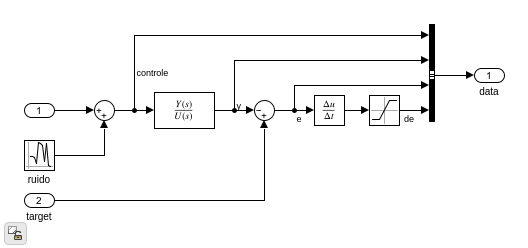
\includegraphics{fig/FT.png}
  \caption{Núcleo da simulação.}
  \label{fig:FT}
\end{figure}

Estando o "centro" da simulação pronto, foram criados os testes usando um bloco \textit{Subsystem reference} em cada um, como mostrado em \ref{fig:modelo}. O primeiro deles não usa controlador, ele é apenas representa a planta em malha aberta, o target é diretamente usado como controle e sua saída é salva na variável \emph{data\_aberto}. O segundo usa um controlador PID com parâmetros $K_p=4$, $K_i=25$ e $K_d=1$ e sua saída é salva na variavél \emph{data\_pid}. Por fim, o terceiro usa o controlador Fuzzy desenvolvido neste trabalho e seu resultado é armazenado em \emph{data\_fuzzy}.

\begin{figure}
  \centering
  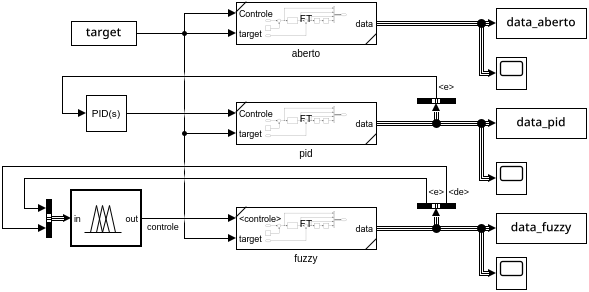
\includegraphics{fig/modelo.png}
  \caption{Simulações em planta aberta, PID e Fuzzy.}
  \label{fig:modelo}
\end{figure}

\section{Controlador Fuzzy}

Foram testadas inúmeras combinações de intervalos e quantidades até que fosse atingido um resultado satisfatório. Sem dúvidas a principal estratégia usada para buscar a melhor combiação de parâmetros foi pensar em como remover o overshoot, evitando que o controlador tentasse corrigir o erro por meio de oscilações que consomem tempo. Assim o controlador resultante pode ser visto nas figuras de \ref{fig:input_1} a \ref{fig:superficie}.

\begin{figure}
  \centering
  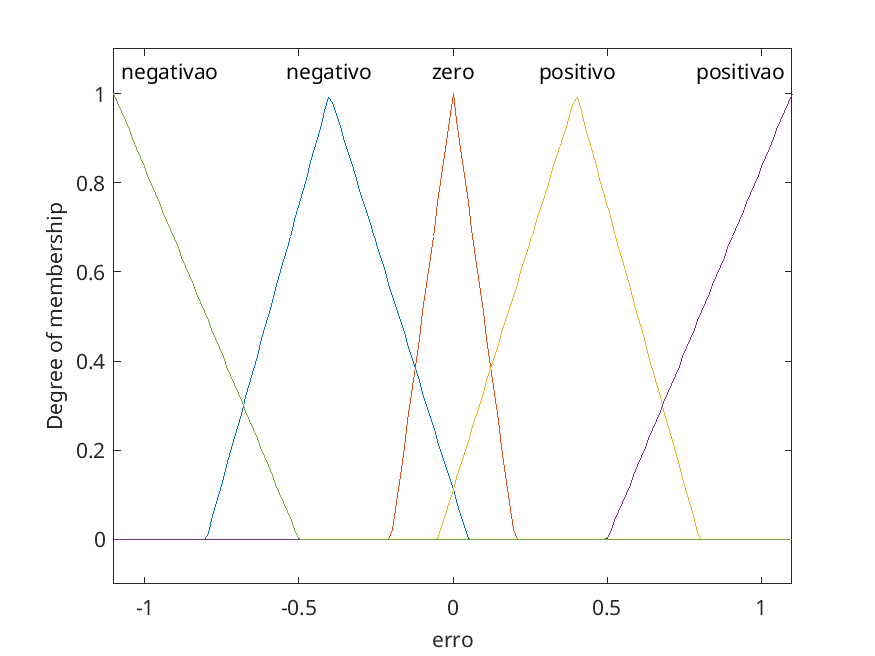
\includegraphics{fig/fuzzy_input_1.png}
  \caption{Funções de pertinência do erro.}
  \label{fig:input_1}
\end{figure}

\begin{figure}
  \centering
  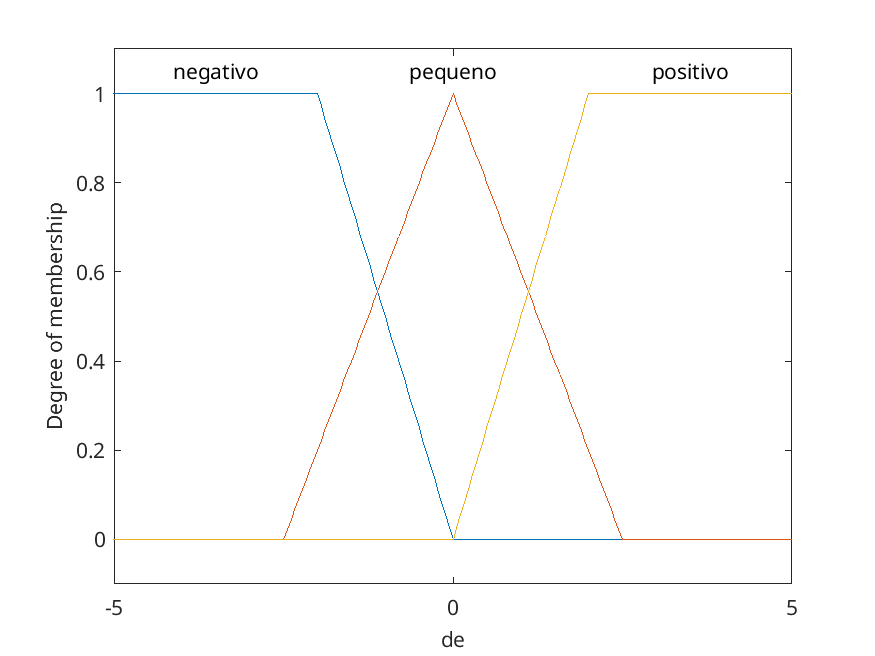
\includegraphics{fig/fuzzy_input_2.png}
  \caption{Funções de pertinência da derivada do erro.}
  \label{fig:input_2}
\end{figure}

\begin{figure}
  \centering
  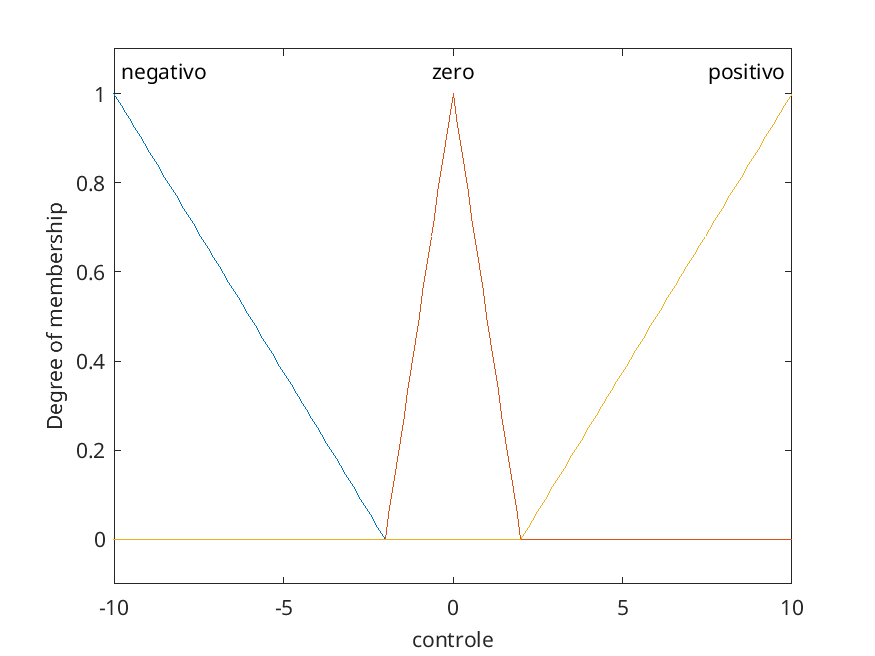
\includegraphics{fig/fuzzy_output.png}
  \caption{Funções de pertinência da saída.}
  \label{fig:output}
\end{figure}

\begin{figure}
  \centering
  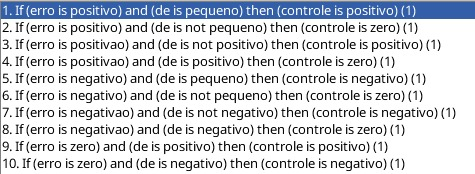
\includegraphics{fig/regras.jpeg}
  \caption{Regras do controlador.}
  \label{fig:regras}
\end{figure}

\begin{figure}
  \centering
  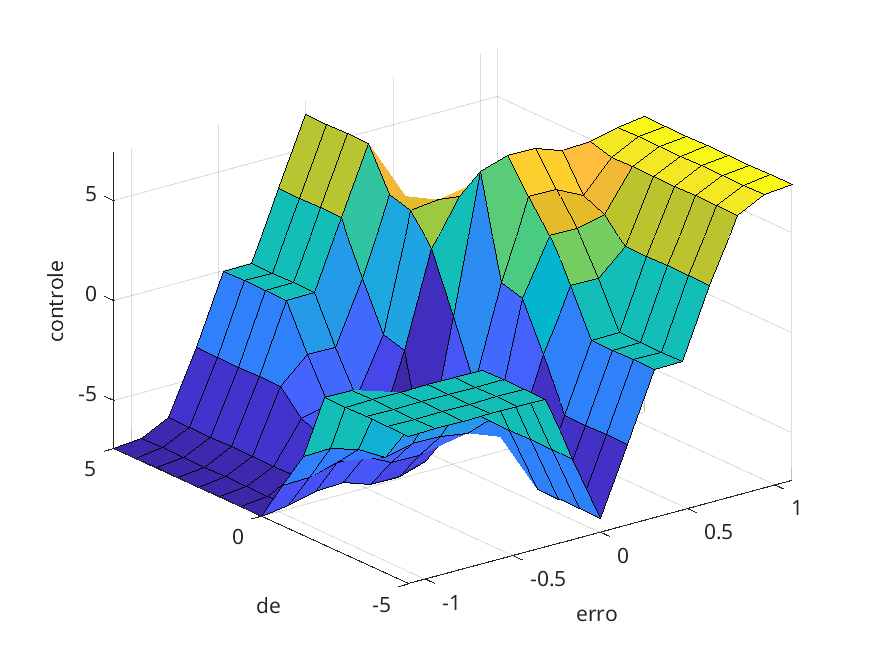
\includegraphics{fig/fuzzy_surface.png}
  \caption{Superfície de controle usada.}
  \label{fig:superficie}
\end{figure}

\section{Simulação com MATLAB}

Muitos testes foram feitos e muitas imagens foram geradas, por isso todo o processo de simulação e geração de figuras foi automatizado usando o código MATLAB.

\lstinputlisting[label=code:principal, caption={Código principal da simulação.}]{principal.m}



\section{Resultados}

\begin{table}
  \centering
  \caption{Resultados obtidos com a planta original e sem ruído.}
  \begin{tblr}{
    cell{1}{1} = {r=2}{},
    vlines,
    hline{1,3-6} = {-}{}}
    Sistema & Tempo de   & Sobre-sinal máximo \\
            & acomodação & percentual         \\
    Aberto  & 1,99 s     & 4,6\%              \\
    PID     & 2,18 s     & 17,8\%             \\
    Fuzzy   & 356 ms     & 0,41\%
  \end{tblr}
  \label{tab:resultados_otimistas}
\end{table}

\printglossary[type=\acronymtype]
\printglossary

\end{document}